\documentclass[border=5pt]{standalone}
\usepackage{tikz}
\usepackage{xcolor}
\usetikzlibrary{positioning,shapes.geometric}

\begin{document}
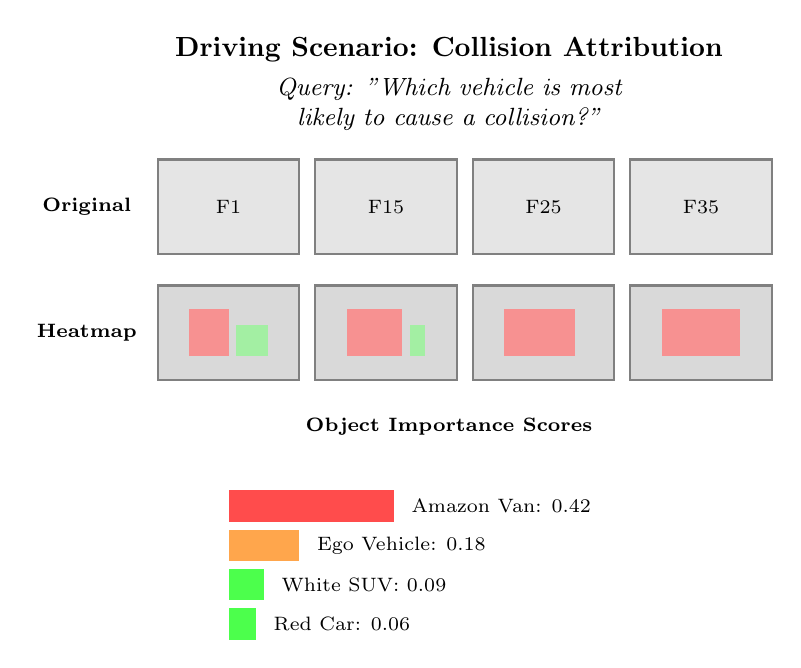
\begin{tikzpicture}[
    frame/.style={draw=gray, thick, minimum width=1.8cm, minimum height=1.2cm, fill=gray!20},
]

% Title
\node[font=\bfseries] at (3.8, 4.2) {Driving Scenario: Collision Attribution};

% Query
\node[font=\small\itshape, text width=8cm, align=center] at (3.8, 3.5) {
    Query: "Which vehicle is most likely to cause a collision?"
};

% Original frames row
\node[font=\scriptsize\bfseries] at (-0.8, 2.2) {Original};
\node[frame] (o1) at (1, 2.2) {\scriptsize F1};
\node[frame] (o2) at (3, 2.2) {\scriptsize F15};
\node[frame] (o3) at (5, 2.2) {\scriptsize F25};
\node[frame] (o4) at (7, 2.2) {\scriptsize F35};

% Heatmap frames row
\node[font=\scriptsize\bfseries] at (-0.8, 0.6) {Heatmap};
\node[frame, fill=gray!30] (h1) at (1, 0.6) {};
\node[frame, fill=gray!30] (h2) at (3, 0.6) {};
\node[frame, fill=gray!30] (h3) at (5, 0.6) {};
\node[frame, fill=gray!30] (h4) at (7, 0.6) {};

% Red highlights for important vehicle
\fill[red!50, opacity=0.8] (0.5, 0.3) rectangle (1.0, 0.9);
\fill[red!50, opacity=0.8] (2.5, 0.3) rectangle (3.2, 0.9);
\fill[red!50, opacity=0.8] (4.5, 0.3) rectangle (5.4, 0.9);
\fill[red!50, opacity=0.8] (6.5, 0.3) rectangle (7.5, 0.9);

% Green for other vehicles
\fill[green!50, opacity=0.6] (1.1, 0.3) rectangle (1.5, 0.7);
\fill[green!50, opacity=0.6] (3.3, 0.3) rectangle (3.5, 0.7);

% Importance bar chart
\node[font=\scriptsize\bfseries] at (3.8, -0.6) {Object Importance Scores};

% Bars
\fill[red!70] (1, -1.8) rectangle (3.1, -1.4);
\fill[orange!70] (1, -2.3) rectangle (1.9, -1.9);
\fill[green!70] (1, -2.8) rectangle (1.45, -2.4);
\fill[green!70] (1, -3.3) rectangle (1.35, -2.9);

% Labels
\node[font=\scriptsize, anchor=west] at (3.2, -1.6) {Amazon Van: 0.42};
\node[font=\scriptsize, anchor=west] at (2.0, -2.1) {Ego Vehicle: 0.18};
\node[font=\scriptsize, anchor=west] at (1.55, -2.6) {White SUV: 0.09};
\node[font=\scriptsize, anchor=west] at (1.45, -3.1) {Red Car: 0.06};

\end{tikzpicture}
\end{document}
